\section{Methodology}
\label{sec:methodology}

\subsection{Conversion Pipeline}
\label{sec:pipeline}

Our conversion toolkit transforms NVIDIA Isaac Sim assets from MDL materials
to UsdPreviewSurface while preserving the compositional structure of USD
scenes. The pipeline operates in three stages.

\begin{figure*}[t]
\centering
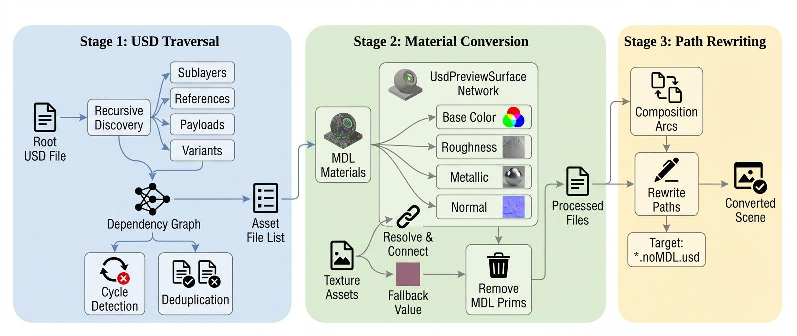
\includegraphics[width=\textwidth]{figures/fig_method_pipeline.pdf}
\caption{Overview of the composition-preserving MDL-to-UsdPreviewSurface conversion pipeline. The processor recursively discovers dependent USD files without flattening the scene composition, converts MDL materials in each file to a minimal UsdPreviewSurface approximation, rewrites composition arcs to sibling \texttt{*\_noMDL.usd} assets, and preserves a self-consistent converted USD hierarchy.}
\label{fig:method_pipeline}
\end{figure*}

Figure~\ref{fig:method_pipeline} summarizes the traversal, conversion, and
rewriting stages that transform an MDL-based USD composition into Preview-only
assets while preserving the original scene structure.

\paragraph{Stage 1: Recursive USD Traversal.}
The processor begins at a root USD file and recursively discovers all
referenced assets --- sublayers, references, payloads, variant selections, and
value clips --- building a dependency graph.  A cycle-detection mechanism
(\texttt{in\_stack} set) prevents infinite recursion on circular references,
while a deduplication dictionary (\texttt{done} map) ensures each asset file is
processed exactly once. Crucially, the pipeline does \emph{not} flatten the USD
composition: each file is processed independently and saved as a sibling
\texttt{*\_noMDL.usd} file, so the original composition arcs (references,
payloads, variants) remain intact with only their asset paths rewritten to
point to the converted counterparts.

\paragraph{Stage 2: Material Conversion.}
For each USD file in the dependency graph, the pipeline identifies all
materials driven by MDL shaders. It constructs a minimal UsdPreviewSurface
shader network per material, mapping four primary channels: base color (diffuse
albedo), roughness, metallic, and normal. Texture assets referenced by the MDL
shader are located, resolved against the declaring layer's directory, and
connected to the new UsdPreviewSurface inputs via \texttt{UsdShadeConnectableAPI}.
When texture files cannot be resolved, constant fallback values are used.
MDL features not captured by the four-channel mapping include subsurface
scattering, clearcoat layers, anisotropic reflectance, emission, opacity, and
displacement. After the UsdPreviewSurface network is established, all MDL shader prims and
MDL-specific material outputs are removed. A post-conversion verification pass
confirms that no MDL residuals remain.

\paragraph{Stage 3: Asset Path Rewriting.}
All composition arcs in the converted file --- references, payloads, sublayer
paths, and variant-internal asset paths --- are rewritten from their original
targets to the corresponding \texttt{*\_noMDL} variants. This ensures that
opening the converted root file yields a fully self-consistent scene composed
entirely of UsdPreviewSurface materials.

\subsection{Experimental Setup}
\label{sec:setup}

\paragraph{Dataset.}
We select four chest-of-drawers assets from the NVIDIA Isaac Sim asset library:
\texttt{chestofdrawers\_0004}, \texttt{chestofdrawers\_0011},
\texttt{chestofdrawers\_0023}, and \texttt{chestofdrawers\_0029}. These objects
feature diverse wood, metal, and fabric materials with varying degrees of MDL
complexity, including multi-layer coatings and procedural textures, making them
representative test cases for material simplification.

\paragraph{Rendering.}
For each object, we render images from six camera viewpoints distributed around
the scene: front, back, left, right, top-front-left, and top-front-right.
Each viewpoint is rendered twice --- once with the original MDL materials and
once with the converted UsdPreviewSurface materials --- yielding $4 \times 6
\times 2 = 48$ images total (24 matched pairs). All renders use identical
geometry, lighting, and camera parameters at $1024 \times 1024$ resolution to
isolate the effect of material representation.

\paragraph{Hardware.}
All experiments are conducted on a workstation equipped with an NVIDIA GeForce
RTX 4090 (24\,GB VRAM) GPU and an Intel Xeon Gold 6462C processor. Rendering uses NVIDIA Isaac Sim's
built-in RTX renderer. Feature extraction runs on the same GPU hardware.

\subsection{Evaluation Metrics}
\label{sec:metrics}

We evaluate the impact of material simplification at three complementary levels.

\paragraph{Rendering Performance.}
We measure scene load time in a headless benchmark by timing
\texttt{open\_stage} plus a fixed 30-update post-open warm-up window, which
approximates the time to a ready-to-render state in our setup. We report this
metric separately for the first cold-start pass and the subsequent warm passes,
together with post-load GPU memory consumption (MB) and steady-state rendering
throughput (frames per second) for both MDL and UsdPreviewSurface versions of
each scene. To better approximate practitioner-facing startup cost at scale, we
also run a supplemental large-scene benchmark on one composed GRScenes
commercial interior, launching a fresh headless Isaac Sim process for each run
and measuring scene-ready time from \texttt{open\_stage} through the same
30-update post-open window.

\paragraph{Pixel-Level Image Quality.}
For each of the 24 matched image pairs, we compute:
\begin{itemize}
    \item \textbf{PSNR} (Peak Signal-to-Noise Ratio): measures pixel-level
    reconstruction accuracy in decibels (higher is better).
    \item \textbf{SSIM}~\cite{Wang2004Image} (Structural Similarity Index):
    captures luminance, contrast, and structural distortion on a $[0,1]$ scale
    (higher is better).
    \item \textbf{LPIPS}~\cite{Zhang2018Unreasonable} (Learned Perceptual
    Image Patch Similarity, VGG backbone): uses deep features to measure
    perceptual distance (lower is better).
\end{itemize}

\paragraph{Feature-Level Preservation.}
To assess whether material simplification alters semantic content as perceived
by modern vision models, we extract embeddings from both
CLIP~\cite{Radford2021Learning} (ViT-B/32) and
DINOv2~\cite{Oquab2023DINOv2} (ViT-B/14) for each matched pair and compute
cosine similarity. High similarity ($> 0.95$) indicates that the feature
representations are largely invariant to the material change. We report
per-pair scores and across-scene averages to identify whether specific material
types are more sensitive to simplification. All reported standard deviations use the sample standard deviation ($n-1$ denominator).

